
Neural network models have become ubiquitous in natural language processing applications, pushing the state-of-the-art in a large variety of tasks involving natural language understanding (NLU) and generation \cite{wu2016google,wang2019superglue}.
In the past year, significant improvements have been obtained by  training increasingly larger neural network language models on huge amounts of data openly available on the web and then fine-tuning those base models for each downstream task \cite{devlin2018bert,peters2018deep,liu2019multi}.

\begin{figure}[tbp]
\centering
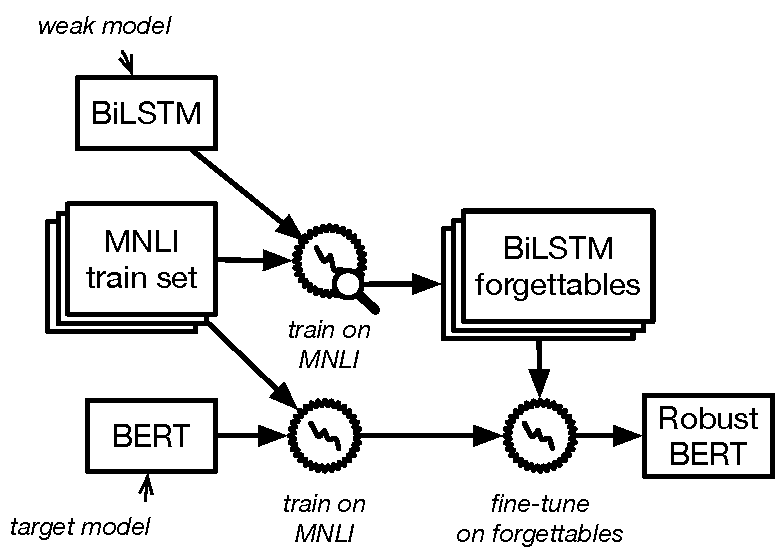
\includegraphics[scale=0.55]{figures/acl.pdf}
\caption{Proposed training for obtaining more robust natural language inference models. We first detect~\emph{forgettable}, or~\emph{hard}, examples from the MNLI training set using a weak model. These are likely to be examples that cannot be solved by simple heuristics. Then, after having fine-tuned a target model on the MNLI training set, we perform an auxiliary round of fine-tuning only on the forgettable subset to obtain a more robust model.}
\label{}
\end{figure}

In spite of their impressive performance, empirical evidence suggests that these models may be far from forming human-like representations of natural language. Their predictions have been shown to be brittle on examples that slightly deviate from the training distribution but are still syntactically and semantically valid \cite{jia2017adversarial,linzen2019right}.
In the context of natural language inference (NLI), increasing evidence supports the hypothesis that these models lack robustness because they mainly tend to capture task- and dataset-specific biases such as shallow lexical word overlap features~\cite{poliak2018hypothesis,dasgupta2018evaluating,linzen2019right,clark2019dont,zhang-etal-2019-paws}. These results are generally obtained by observing a drop in performance when testing highly performant NLI models, for example trained on MNLI~\citep{williams2017broad}, on datasets containing examples for which shallow lexical features are not predictive of class labels,~e.g. HANS~\citep{linzen2019right}. These datasets contain under-represented modes of the ground-truth distribution and the desiderata is to train NLI models which are more robust to such distribution shifts.

In this paper, we investigate the possibility of identifying a set of \emph{hard}, or \emph{atypical}, examples which would unlikely be explained by simple heuristics and, if identified correctly and up-weighted during training, could enable learning of more robust features which would compensate for distribution shift~\citep{sugiyama2007covariate}.
% Here, we explore whether examples considered hard by \emph{simpler} models\footnote{Parametric models with a small number of parameters.} naturally exclude the dataset's heuristics without any prior knowledge of them. 
We consider example forgetting~\cite{toneva2018empirical} as a model-dependent measure of hardness of an example. This metric considers an example hard, or \emph{forgettable}, both when it fluctuates between being learnt or unlearnt during training (i.e., it is close to the decision boundary between classes), and when it has never been learnt before the end of training (i.e., it is possibly out of distribution), thus encompassing the dynamics of example learning, and not solely its loss at the end of training, as considered in~\newcite{clark2019dont}.

Recently, \newcite{clark2019dont,mahabadi2019simple} give evidence towards the effectiveness of re-weighting training examples for increasing robustness but they  generally assume~\emph{a priori} knowledge of the heuristics present in the dataset. 
Here, we show that it suffices to consider hard examples by~\emph{simpler} models\footnote{We consider a model simple if it has a small number of parameters.} which seem to naturally exclude the dataset's heuristics without any prior knowledge of them. We do not make a conscious effort in designing the simpler models based on known heuristics. The underlying assumption is that simpler models capture more easily simple explanations of the training data but tend to underfit complex patterns. We investigate whether up-weighting forgettable examples under such simple models can help in training more robust models.

% We also investigate whether increased robustness to out-of-distribution examples could come \emph{for free} when training larger, more performant NLI models. To this end, we compare the performance 
% For a given task (\textit{e.g.} image classification), example forgetting is defined as the number of times the neural network shifts from properly classifying an example to making a mistake on the same example at the next training epoch. Examples with at least one forgetting event, the \emph{forgettable} examples, are rather atypical compared to the \emph{unforgettable} ones that contain very common features, prototypical of the class (\textit{e.g.} an occluded gray plane versus a white plane centered on a bright blue sky). It is interesting to note that forgetting events capture the dynamics of example learning, and not solely their loss at the end of training, as considered in \newcite{clark2019dont}. In this paper, we investigate whether up-weighting forgettable (aka hard) examples can help in training more robust models.

% We consider~\emph{example forgetting} \cite{toneva2018empirical} as a model-dependent measure of ``hardness'' of an example. For a given task (\textit{e.g.} image classification), example forgetting is defined as the number of times the neural network shifts from properly classifying an example to making a mistake on the same example at the next training epoch. Examples with at least one forgetting event, the \emph{forgettable} examples, are rather atypical compared to the \emph{unforgettable} ones that contain very common features, prototypical of the class (\textit{e.g.} an occluded gray plane versus a white plane centered on a bright blue sky). In this paper, we investigate whether up-weighting forgettable (aka hard) examples can help in training more robust models.  

% Our main contributions are:
% \begin{itemize}
Our first contribution is to extend the results of~\newcite{toneva2018empirical} by detecting forgettable examples in MNLI~\cite{williams2017broad} and QQP~\cite{qqp}, a paraphrase dataset, for various architectures of increasing capacity. Training NLI models on forgettable examples only leads to poor performance, a fact which contrasts with the observations by~\newcite{toneva2018empirical} in the image setting.
% Our results show that weaker models tend to overfit on known heuristics for those datasets, a fact which contrasts with the observations by~\newcite{toneva2018empirical} in the image setting, and open paths for future investigations.

Then, we propose a new training method to increase the robustness of NLP models, consisting in fine-tuning models on the subset of forgettable examples of simpler models. Our approach does not assume~\emph{a priori} knowledge about the existing heuristics in the datasets. We apply our method to BERT~\citep{devlin2018bert} and XLNET~\citep{yang2019xlnet} models and demonstrate a significant gain in robustness: our best models achieve better performance than BERT, XLNET and recently proposed robust models. 
% on HANS~\citep{linzen2019right} and PAWS~\citep{zhang-etal-2019-paws}.
\enote{yy}{Above: the PAWS citation isn't proposing robust model.}

% \item 
% \enote{yy}{ThIS IS REPEATED: We apply our method to both \emph{base} and \emph{large} versions of recently proposed BERT~\citep{devlin2018bert} and XLNET~\citep{yang2019xlnet} models to measure the effect of example re-weighting under different model capacities.}
Finally, we show that the \emph{large} versions of BERT and XLNET outperform their base counterparts on HANS and PAWS~\citep{zhang-etal-2019-paws}, demonstrating that larger models are more robust and that they can also be improved by our method. For instance, \xlnetlarge goes from 76.1\% to 83.1\% on HANS. To the best of our knowledge, these are the first evaluations on HANS of \bertlarge and XLNET\footnote{We will release our code
as part of publication.}.
% \end{itemize}

% We first extend the results of \newcite{toneva2018empirical} by computing forgetting events in MNLI \cite{williams2017broad}, a natural language inference dataset, and QQP \cite{qqp}, a paraphrase dataset, for various architectures of increasing capacity. The robustness of our models is verified by considering their performance on the recently proposed HANS and PAWS test sets. HANS \cite{linzen2019right} contains linguistically correct inference problems that cannot be solved by simple common heuristics, such as lexical overlap, usually learnt by models trained on the MNLI training set. Similarly, PAWS \cite{zhang-etal-2019-paws} contains paraphrase and non-paraphrase pairs with high lexical overlap, and is extremely challenging for models trained on the QQP training set. Our best models achieve better performance on the HANS and PAWS datasets than BERT, XLNET and recently proposed robust models. We also uncover interesting insights on forgettable examples for these datasets, which contrast with the observations by \newcite{toneva2018empirical} in the image setting, and open paths for future investigations.

% We first extend the results of \newcite{toneva2018empirical} by computing forgetting events in MNLI \cite{williams2017broad}, a natural language inference dataset, and QQP \cite{qqp}, a paraphrase dataset, for various architectures of increasing capacity. The robustness of our models is verified by considering their performance on the recently proposed HANS and PAWS test sets. HANS \cite{linzen2019right} contains linguistically correct inference problems that cannot be solved by simple common heuristics, such as lexical overlap, usually learnt by models trained on the MNLI training set. Similarly, PAWS \cite{zhang-etal-2019-paws} contains paraphrase and non-paraphrase pairs with high lexical overlap, and is extremely challenging for models trained on the QQP training set. Our best models achieve better performance on the HANS and PAWS datasets than BERT, XLNET and recently proposed robust models. We also uncover interesting insights on forgettable examples for these datasets, which contrast with the observations by \newcite{toneva2018empirical} in the image setting, and open paths for future investigations.

% Each such occurrence is coined a \emph{forgetting event}.
% The authors show that on various image datasets, the distribution of forgetting events is rather striking: numerous examples are never forgotten -- that is, once properly classified they remain so for the rest of training, while others withstand many a forgetting event.
% Visually inspecting those \emph{forgettable examples} shows they are rather atypical compared to the \emph{unforgettable} ones that are fairly prototypical of a class (\textit{e.g.} an occluded gray plane versus a white plane centered on a bright blue sky).
 


